%% PEV & other internshis' style for LaTeX2e
%% 
%% FEUP, JCL, Thu Dec 14 15:23:03 2023
%%
%% PLEASE send improvements to jlopes at fe.up.pt

\documentclass[11pt,a4paper]{report}

%%------------------------------- preamble ------------------------------------

%% comment next for EN
\usepackage[portuges]{babel}      % language PT 
\usepackage[utf8]{inputenc}       % accents
\usepackage[T1]{fontenc}          % PS fonts
\usepackage{newtx}                % do not use CM fonts
\usepackage{amsmath}              % multi-line and other mathematical statements,
\usepackage{setspace}             % setting the spacing between lines
\usepackage{graphicx}             % go far beyond what the graphics package
\usepackage[normalem]{ulem}       % various types of underlining
\usepackage{caption}              % rotating captions, sideways captions, etc.
\usepackage{float}                % tables and figures in the multi-column environment 
\usepackage{subcaption}           % for subfigures and the like
\usepackage{longtable}            % tables that continue to the next page
\usepackage{multirow}             % tabular cells spanning multiple rows
\usepackage[table]{xcolor}        % driver-independent color extensions
\usepackage{lipsum}               % loren dummy text
\setlength{\marginparwidth}{2cm}  % todonotes' requirements
\usepackage{todonotes}            % todo's
\usepackage{chicago}              % a bibliography style

%% document dimensions
\usepackage[a4paper, left=25mm, right=25mm, top=25mm, bottom=25mm,
   headheight=6mm, footskip=12mm]{geometry}
\setlength{\parindent}{0em}
\setlength{\parskip}{1ex}

%% headers & footers
\usepackage{lastpage}
\usepackage{fancyhdr}
\fancyhf{}                            % clear off all default fancyhdr headers and footers
\rhead{\small{\emph{\projtitle, \projauthor}}}
\rfoot{\small{\thepage\ / \pageref{LastPage}}}
\pagestyle{fancy}                     % apply the fancy header style
\renewcommand{\headrulewidth}{0.4pt}
\renewcommand{\footrulewidth}{0.4pt}

%% colors
\usepackage{color}
\definecolor{engineering}{rgb}{0.549, 0.176, 0.098}
\definecolor{cloudwhite}{cmyk}{0,0,0,0.025}

%% source-code listings
\usepackage{listings}
\lstset{ %
 language=C,                        % choose the language of the code
 basicstyle=\footnotesize\ttfamily,
 keywordstyle=\bfseries,
 numbers=left,                      % where to put the line-numbers
 numberstyle=\scriptsize\texttt,    % the size of the fonts that are used for the line-numbers
 stepnumber=1,                      % the step between two line-numbers. If it's 1 each line will be numbered
 numbersep=8pt,                     % how far the line-numbers are from the code
 frame=tb,
 float=htb,
 aboveskip=8mm,
 belowskip=4mm,
 backgroundcolor=\color{cloudwhite},
 showspaces=false,                  % show spaces adding particular underscores
 showstringspaces=false,            % underline spaces within strings
 showtabs=false,                    % show tabs within strings adding particular underscores
 tabsize=2,                         % sets default tabsize to 2 spaces
 captionpos=b,                      % sets the caption-position to bottom
 breaklines=true,                   % sets automatic line breaking
 breakatwhitespace=false,           % sets if automatic breaks should only happen at whitespace
 escapeinside={\%*}{*)},            % if you want to add a comment within your code
 morekeywords={*,var,template,new}  % if you want to add more keywords to the set
}

%% hyperreferences (HREF, URL)
\usepackage{hyperref}
\hypersetup{
    plainpages=false, 
    pdfpagelayout=SinglePage,
    bookmarksopen=false,
    bookmarksnumbered=true,
    breaklinks=true,
    linktocpage,
    colorlinks=true,
    linkcolor=engineering,
    urlcolor=engineering,
    filecolor=engineering,
    citecolor=engineering,
    allcolors=engineering
}

%% path to the figures directory
\graphicspath{{figures/}}

%% macros, to be updated as needed
\newcommand{\school}{Faculdade de Engenharia da Universidade do Porto}
\newcommand{\degree}{Licenciatura em Engenharia Informática e Computação}
\newcommand{\projtitle}{Título do Trabalho}
\newcommand{\company}{Nome da Empresa}
\newcommand{\projauthor}{Nome do Autor}
\newcommand{\supervisor}{Nome do Supervisor}
\newcommand{\tutor}{Prof.\ João Correia Lopes}

%% my other macros, if needed
\newcommand{\windspt}{\textsf{WindsPT\/}}
\newcommand{\windscannerpt}{\emph{Windscanner.PT\/}}
\newcommand{\class}[1]{{\normalfont\slshape #1\/}}
\newcommand{\svg}{\class{SVG}}

%% my environments for infos
\newenvironment{info}[1]{\vspace*{6mm}\color{blue}[ \textbf{INFO:} \begin{em} #1}
                        {\vspace*{3mm}\end{em} ]}
\newenvironment{infoopt}[1]{\vspace*{6mm}\color{blue}[ \textbf{INFO (elemento opcional):} \begin{em} #1}
                        {\vspace*{3mm}\end{em} ]}

%%------------------------------- document-------------------------------------

\begin{document}

%% preamble with (reseted) roman page numbers
\pagenumbering{roman}\setcounter{page}{1}

%%------------------------------- cover page ----------------------------------

\begin{titlepage}
\center

\vspace{-15mm}
{\Large \textbf{\textsc{\school}}}\\[28mm]

{\huge \textbf{\projtitle}}\\[8mm]
{\huge \textbf{\company}}\\[30mm]

{\Large \textbf{\projauthor}}\\[56mm]


\includegraphics[width=70mm]{uporto-feup.pdf}\\[30mm]

{\large \degree}\\[12mm]
{\large Supervisor: \supervisor}\\[4mm]
{\large Tutor: \tutor}\\[12mm]

%\renewcommand{\today}{15 de dezembro de 2023}
\today

\end{titlepage}

%%------------------------------- Abstract ------------------------------------

\chapter*{Resumo}

\begin{info}
O resumo tem um caráter essencialmente informativo, devendo ser
escrito de forma concisa (até 200 palavras) de maneira a captar o
interesse de quem o vai ler.

O Resumo substitui a leitura do documento e não contem figuras,
tabelas, citações, etc.\ 
Deve incluir os seguintes tópicos: âmbito, objetivos, os métodos, as
principais descobertas, incluindo resultados, conclusões e
recomendações, se existirem.

Para saber mais sobre como redigir um bom resumo consulte o tutorial
online disponível no website na Biblioteca, ``Guia de Apoio à
Publicação'', secção: 
``\href{https://docs.google.com/document/d/1TDC1behVq8x7fQL4CcPEEh_np5GXviJevQxnQ9gbiJs/edit\#heading=h.s4z9k57ywd9w}
{Estruturar Relatório Técnico}''.
\end{info}

\todo[inline]{Escrever o Resumo, mas só no fim.}

%\vspace{\fill}
%{\Large \textbf{Palavras-chave}:} palavra1, palavra2, palavra3, palavra4
%\vspace*{24mm}

%%------------------------------- Acknowledgments -----------------------------

\chapter*{Agradecimentos}

\begin{infoopt}
Habitualmente é mencionada a contribuição de outras pessoas ou
entidades, tanto para a realização do estudo como para a produção do
relatório. 
Podem fazer-se numa página autónoma ou incluir-se na introdução.
\end{infoopt}

%%------------------------------- table of contents ---------------------------

\tableofcontents

%%------------------------------- list of todos -------------------------------

% list todos; comment in the end (should be empty before delivery :-)
\listoftodos

\begin{infoopt}
Podem ser colocadas anotações durante a preparação do documento, que
são listadas aqui.

Este elemento não aparece no documento final!
\end{infoopt}

%%------------------------------- list of figures -----------------------------

\listoffigures
%\addcontentsline{toc}{chapter}{Lista de figuras}

\begin{infoopt}
Justifica-se quando é necessário apresentar elementos complementares à
compreensão do texto (fotografias, tabelas, gráficos, etc.), que devem
ser previamente identificados sob a forma de listas, com as respetivas
legendas e páginas de início. 
\end{infoopt}

%%------------------------------- list of tables ------------------------------

\listoftables
%\addcontentsline{toc}{chapter}{Lista de tabelas}

\begin{infoopt}
Justifica-se quando é necessário apresentar,  na forma tabular,
elementos complementares à compreensão do texto.
\end{infoopt}

%%------------------------------- Acronyms ------------------------------------

\chapter*{Lista de acrónimos}
%\addcontentsline{toc}{chapter}{Lista de acrónimos}

\begin{flushleft}
\begin{tabular}{l p{0.8\linewidth}}
ADT      & Abstract Data Type\\
API      & Application Programming Interface\\
WWW      & World Wide Web
\end{tabular}
\end{flushleft}

\begin{infoopt}
Justifica-se se estes elementos (acrónimos, unidades, símbolos)
ocorrerem com grande frequência no relatório.

Quando ocorrerem pela primeira vez no texto deve apresentar-se a
respetiva definição.
Por exemplo: Application Programming Interface (ADT) é uma \ldots 

A lista de itens deve ser ordenada alfabeticamente.
\end{infoopt}

%%------------------------------- Glossary ------------------------------------

\chapter*{Glossário}
\addcontentsline{toc}{chapter}{Glossário}

\begin{description}
\item[bash] \hfill \\
  Bash é uma \emph{shell Unix} e uma linguagem de comando escrita 
  em 1989 por Brian Fox para o Projeto GNU como um substituto de 
  software livre para a \emph{Bourne shell}.
\item[firewall] \hfill \\
  Em computação, uma \emph{firewall} é um sistema de segurança de rede 
  que monitoriza e controla o tráfego de entrada e saída da rede 
  com base em regras de segurança predeterminadas.
  Uma \emph{firewall} normalmente estabelece uma barreira entre uma 
  rede confiável e uma rede não confiável, como a Internet.
\item[Glossário] \hfill \\
  Glossário é uma espécie de pequeno dicionário específico para
  palavras e expressões pouco conhecidas presentes num texto, seja
  por serem de natureza técnica, regional ou de outro idioma.
\end{description}

\begin{infoopt}
Justifica-se sempre que seja necessário esclarecer o leitor sobre o
significado de terminologia específica usada no texto no relatório.
Recomenda-se a sua localização nos elementos iniciais, embora na
normalização existente haja variantes, podendo também constar nos
elementos finais.

A lista de itens deve ser ordenada alfabeticamente.

Para saber mais consulte o tutorial online 
``\href{https://docs.google.com/document/d/1TDC1behVq8x7fQL4CcPEEh_np5GXviJevQxnQ9gbiJs/edit}
{Guia de Apoio à Publicação}''.
\end{infoopt}

%%------------------------------- chapter ------------------------------------

\chapter{Introdução}

\pagestyle{fancy}
% reset and change to roman page numbers
\pagenumbering{arabic}\setcounter{page}{1}

\begin{info}
Contextualização sucinta do assunto do relatório, fazendo-se
referência ao âmbito e aos objetivos.
Aqui se clarifica a motivação do trabalho apresentado e se explica a
abordagem adotada e a sua relação com trabalhos análogos, numa
perspetiva genérica.
Não se deve antecipar detalhes sobre o que é explicado nas secções
posteriores. 
Se for pertinente, pode-se indicar ainda qual o público a que se
destina.

Para saber mais consulte o tutorial online 
``\href{https://docs.google.com/document/d/1TDC1behVq8x7fQL4CcPEEh_np5GXviJevQxnQ9gbiJs/edit}
{Guia de Apoio à Publicação}''.
\end{info}

\section{Contexto}

\begin{info}
Apresentar o contexto organizacional em que decorreu o projeto/estágio (empresa).
\end{info}

\section{Problema}

\begin{info}
Apresentar o problema abordado e a motivação para o trabalho
realizado (qual é o problema abordado e porque é que é importante).
\end{info}

\section{Objetivos e Resultados}

\begin{info}
Indicar os objetivos do trabalho e os resultados esperados.
\end{info}

%%------------------------------- DELETEME

\newpage  % don't do this
\section*{Exemplos}

\begin{info}
  São ilustradas de seguida algumas partes do documento.
  
  Esta secção não aparece no documento final!
\end{info}

\subsection*{Equações}

\begin{info}
Este texto é apenas um exemplo que precede uma equação.
\end{info}  

Equações simples podem ser inseridas em linha com o texto: 
a reta é \(y=mx+b\).

Equações mais complicadas devem ser separadas em linhas individuais e
numeradas sequencialmente à direita dentro de parêntesis.
Esta é a equação 2º grau genérica:

\begin{equation} \label{eq:1}
  ax^2+bx+cx=0
\end{equation}

Onde $a$ é o coeficiente de 2º grau; $b$ o de 1º grau; $c$ o
coeficiente independente da variável $x$, a determinar.

As equações devem ser referidas mantendo o seu número.
Por exemplo, a Equação~\ref{eq:2} resolve problemas formulados tal como 
mostrado na Equação~\ref{eq:1}.

\begin{equation} \label{eq:2}
  x=\frac{-b\pm \sqrt{b^2-4ac}}{2a}
\end{equation}

\subsection*{Figuras e tabelas}

Todas as figuras e tabelas devem ser obrigatoriamente legendadas e
numeradas sequencialmente:

\begin{itemize}
\item as figuras devem ser legendadas por baixo;
\item as tabelas devem ser legendadas no topo. 
\end{itemize}

Mantenha as figuras centradas e em linha com o texto para que a
legenda apareça sempre colada com a imagem.

\begin{info}
As figuras devem flutuar livremente na página e ser referidas e
descritas no texto, com as fontes devidamente explicitadas, para
evitar o plágio.
\end{info}

Como exemplo, a Figura~\ref{fig:campus} (retirada de
\url{www.fe.up.pt}) mostra o \emph{campus} da FEUP. 

\lipsum[4]

\begin{figure}
\centering
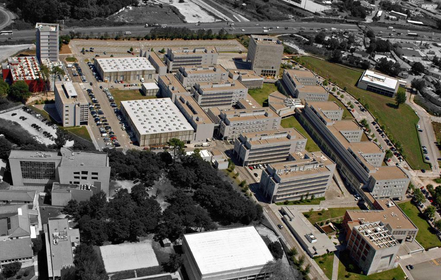
\includegraphics[width=0.72\textwidth]{campus}
\caption{Fotografia aérea do Campus da FEUP.} \label{fig:campus}
\end{figure}

\lipsum[4]

\begin{info}
Pode ser reservado espaço para colocar, no futuro, uma figura; por
exemplo, a Figura~\ref{fig:natal}.
\end{info}

\lipsum[4]

\begin{figure} [b]
  \centering
  \missingfigure{Inserir a figura do Natal.}
  \caption{O Natal no Campus da FEUP.} \label{fig:natal}
\end{figure}

\lipsum[4]

\begin{info}
As tabelas devem flutuar livremente na página e ser referidas e
descritas no texto, com as fontes devidamente explicitadas, para
evitar o plágio.
\end{info}

A Tabela~\ref{tab:feup} (excerto adaptado de ``A FEUP em números'', 2011)
serve para exemplificar como mostrar alguns valores que neste caso têm
a ver com alguns dados numéricos associados a recursos e investimentos
da FEUP no ano de 2011. 

\lipsum[4]

\begin{table}
  \centering
  \caption{Recursos Físicos da FEUP}
  \begin{tabular}{| l | c |}
    \hline
    \textbf{Designação} & \textbf{Quantidade}\\\hline
    \hline
    Área total do campus FEUP & 93 918 $m^2$\\\hline
    Espaços verdes & 23 000 $m^2$\\\hline
    Número de computadores dedicados ao ensino & 1 815\\\hline
    Investimento em equipamentos de laboratório & 1,46 M€\\
    \hline
  \end{tabular}
  \label{tab:feup}
\end{table}

\lipsum[4]

\subsection*{Citações}

À medida que escreve o texto do relatório, deve indicar os trabalhos
de outros autores em que se baseia, sob a forma de citações.
Isto consiste em indicar de forma abreviada as fontes usadas às quais
foi buscar informação adicional para desenvolver o tema do seu
relatório.

Existem duas formas principais de citar:
\begin{itemize}
\item por \textbf{paráfrase}: interpretação do conteúdo original por
  palavras diferentes das da fonte consultada, indicando a fonte logo
  a seguir; ou 
\item 
  por \textbf{transcrição}: uso de um excerto do conteúdo original
  apresentando-o entre aspas, indicando a fonte logo a seguir.
\end{itemize}

As citações devem obedecer a um estilo normalizado.
De entre os muitos que existem, a Biblioteca da FEUP aconselha o
estilo Chicago (formato autor-data).

\begin{info}
De seguida exemplificam-se, ao acaso, algumas citações (por paráfrase)
de acordo com esse estilo.
\end{info}

A decisão de escolha de um tema para um trabalho académico pode
variar~\cite{kn:Bel02-book}.
O tema pode ser pensado e escolhido pelo próprio estudante, ou a
partir de uma lista de temas já concebidos, com potencial interesse
para estudo~\cite{kn:GLPR14-joPhysics}.

A cada citação ao longo do texto deve corresponder uma referência
indicada na lista final de referências
bibliográficas~\cite{kn:Lip08,kn:MSS+12-wemep,kn:VKL+18-dtu}. 

É importante não esquecer que também as figuras (imagens, tabelas,
gráficos, etc.) provenientes de obras de outros autores (por exemplo 
obtidas através da Internet) devem ser citadas sempre, após as
respetivas legendas~\cite{kn:GLPC22-torque}.

Para saber mais sobre este assunto e ver exemplos, consulte o guia
``Evitar o plágio: boas práticas no uso da
informação''\footnote{\url{https://feup.libguides.com/plagio/citar}}.  

\lipsum[4]

\subsection*{Código}

\begin{info}
De seguida é ilustrado como incluir código no documento.
\end{info}

\lipsum[4]

\begin{lstlisting}[language=Python, caption=Python example]
# take the users input
words = input("Enter the text to translate to pig latin: ")
print(f"You entered: {words}")

# now, break apart the words into a list
words = words.split(' ')

# let's use the list to translate words greater than 3 characteres
for i in words:
    if len(i) >= 3:
        i = i + "%say" % (i[0])
        i = i[1:]
        print(i)
    else:
        pass
\end{lstlisting}

\subsection*{Uso das macros}

\begin{info}
De seguida é ilustrada a utlização de macros \LaTeX{} definidas no
preâmbulo.
\end{info}

O \windspt, retirado do \windscannerpt, usa o \svg\ \ldots

\lipsum[2]

\begin{info}
As partes componentes subsequentes que constituem o corpo do texto
devem ser estruturadas em secções, estimando-se que até 3 níveis seja
o suficiente para este tipo de trabalho.

Para saber mais consulte o tutorial online 
``\href{https://docs.google.com/document/d/1TDC1behVq8x7fQL4CcPEEh_np5GXviJevQxnQ9gbiJs/edit}
{Guia de Apoio à Publicação}''.
Note-se que as seções aí indicadas podem ser adaptadas em função do tema
ou profundidade do estudo a desenvolver.

Não é costume haver cabeçalhos de secções seguidas sem texto.
\end{info}


%%------------------------------- chapter ------------------------------------

\chapter{Metodologia}

Neste capítulo é descrita a metodologia seguida, são enumerados os
principais intervenientes no projeto e é feito o registo das
principais atividades desenvolvidas.

\section{Metodologia utilizada}

\begin{info}
Descrever a metodologia seguida (exemplo: desenvolvimento iterativo
com \emph{sprints} quinzenais e reuniões semanais de acompanhamento) e
recursos utilizados (exemplo: GitHub, etc.).
\end{info}

\section{Intervenientes, papéis e responsabilidades}

\begin{info}
Identificar a equipa de projeto, \emph{stakeholders} e outros
intervenientes com os quais existiu interação; no caso de trabalho em
grupo, clarificar os papéis e responsabilidades de cada elemento do grupo.
\end{info}

\section{Atividades desenvolvidas}

\begin{info}
Descrever as atividades realizadas ao longo do tempo (incluindo
eventos relevantes, como apresentações, reuniões com clientes, etc.)
e entregas efetuadas (\emph{deliverables}), recorrendo tipicamente a
um diagrama de Gantt e a uma descrição sumária de cada
atividade/entregável.
Pode ser apresentado também através de tabela com progresso semanal.
\end{info}

%%------------------------------- chapter ------------------------------------

\chapter{Desenvolvimento da solução}

Neste capítulo é descrito o trabalho desenvolvido para alcançar os
resultados esperados.

No caso de um protótipo de software são apresentados os requisitos, a
arquitetura da solução, o desenvolvimento e a validação do protótipo.

\section{Requisitos}

\begin{info}
Requisitos e restrições: identificar os requisitos funcionais e não
funcionais relevantes e respetivas fontes, bem como restrições ao projeto. 
\end{info}

\section{Arquitetura e tecnologias}

\begin{info}
Arquitetura e tecnologias (ou Conceção e Implementação): arquitetura e
tecnologias utilizadas e respetiva justificação (tendo em conta
requisitos e alternativas existentes), diagramas técnicos elaborados,
dificuldades técnicas encontradas e sua resolução, etc. 
\end{info}

\section{Solução desenvolvida}

\begin{info}
Solução desenvolvida: apresentar a solução desenvolvida na ótica do
utilizador, com ajuda de \emph{screenshots}, seguindo um fluxo lógico
de utilização com dados realistas.
\end{info}

\section{Validação}

\begin{info}
Validação: descrever as ações realizadas para validar a solução
desenvolvida, em relação aos requisitos e restrições identificados, e 
respectivos resultados (por exemplo, resultados de avaliação
experimental, testes efetuados, \emph{feedback} de utilizadores ou
especialistas, etc.). 
\end{info}

%%------------------------------- chapter ------------------------------------

\chapter{Conclusões}

\begin{info}
Sumariar os \textbf{resultados alcançados} e as contribuições (em
relação aos objetivos do trabalho).

No caso de trabalho em grupo, clarificar as \textbf{contribuições
  individuais}, em termos qualitativos e quantitativos (percentagem).

Refletir sobre as \textbf{lições aprendidas} (tendo em conta os
objetivos de aprendizagem).

Identificar limitações do trabalho realizado e ideias de melhorias e
\textbf{trabalho futuro}. 
\end{info}


%%------------------------------- Bibliography --------------------------------

\renewcommand{\bibname}{Referências bibliográficas}
\bibliographystyle{chicago}
\bibliography{refs}
\addcontentsline{toc}{chapter}{\refname}  % add it to table of contents

\begin{info}
Na lista final de referências devem constar os trabalhos dos autores
citados de forma abreviada ao longo do texto, obtida automaticamente
com o \class{BibTeX}.
A referência bibliográfica é a forma mais desenvolvida de indicar as
fontes de informação em que se baseou. 
\end{info}

%%------------------------------- appendix ------------------------------------

\appendix
\chapter{Um Apêndice}

\begin{infoopt}
Os apêndices e os anexos contêm informação que complementa, apoia e
clarifica o relatório e cuja inclusão no corpo principal do relatório
interferiria com uma boa ordem de apresentação das ideias.

Há uma diferença importante entre apêndices e anexos.

Para saber mais consulte o tutorial online 
``\href{https://docs.google.com/document/d/1TDC1behVq8x7fQL4CcPEEh_np5GXviJevQxnQ9gbiJs/edit}
{Guia de Apoio à Publicação}''.
\end{infoopt}

%%------------------------------- the end. ------------------------------------

\end{document}
